\def\layersep{2.5cm}
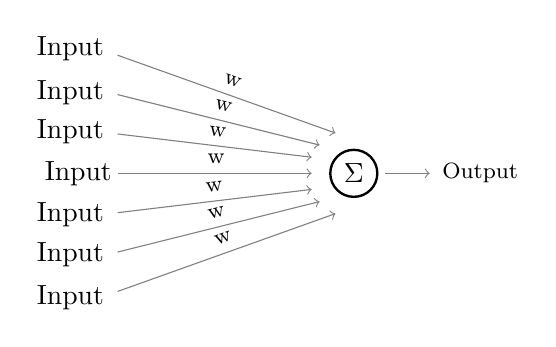
\begin{tikzpicture}[shorten >=1pt,->,draw=black!50, node distance=\layersep]
    \tikzstyle{every pin edge}=[<-,shorten <=1pt]
    \tikzstyle{neuron}=[circle,line width=0.3mm,draw=black,minimum size=17pt,inner sep=0pt]
    \tikzstyle{annot} = [text width=4em, text centered]


    \draw[->] (-3,1.5) -- (-.2,.5) node[sloped,midway,above] {\footnotesize w} node[left=3.4cm,above=.8cm]{Input};
    \draw[->] (-3,1) -- (-.4,.35) node[sloped,midway,above] {\footnotesize w} node[left=3.2cm,above=.4cm]{Input};
    \draw[->] (-3,0.5) -- (-.5,.2) node[sloped,midway,above] {\footnotesize w} node[left=3.1cm,above=.05cm]{Input};
    \draw[->] (-3,0) -- (-.5,0) node[sloped,midway,above] {\footnotesize w} node[left=2.45cm]{Input};
    \draw[->] (-3,-0.5) -- (-.5,-.2) node[sloped,midway,above] {\footnotesize w} node[left=3.1cm,below=.05cm]{Input};
    \draw[->] (-3,-1) -- (-.4,-.35) node[sloped,midway,above] {\footnotesize w} node[left=3.2cm,below=.4cm]{Input};
    \draw[->] (-3,-1.5) -- (-.2,-.5) node[sloped,midway,above] {\footnotesize w} node[left=3.4cm,below=.8cm]{Input};
    
    \node[neuron] (0,0) {$\Sigma$};

    \draw[->] (.4,0) -- (1,0) node[right] {\footnotesize Output};
\end{tikzpicture}